\section{Dateisysteme-API}
%\subsection{Logische Organisation}
%Logische Datei: verwaltete Einheit von Bytes, Inhalt/interne Struktur egal
%Dateiattribute: sichtbar: Dateiname, Grösse, Verzeichnis, Datum des Erstellers, nicht sichtbar: Ablageort/Verkettung von Blöcken auf Datenträger
%\subsection{Dateitypen}
%Applikation muss: sich gegen Datenmüll/Fehlintepretation schützen | nicht annehmen, dass Daten gültig sind | Daten validieren/auf Grenzverletzungen überprüfen
%\subsection{Verzeichnisse}
%Datei, die alle Dateien/Unterverzeichnisse auflistet\\
%root directory hat keinen Namen
\subsubsection{Referenzen}
\prgc{.}$\rightarrow$ auf sich selbst, \prgc{..}$\rightarrow$ auf Elternverzeichnis\\
Jeder Prozess hat Arbeitsverzeichnis. Bezugspunkt für relative Pfade. Wird von aussen festgelegt.
%\prgc{getcwd} $\rightarrow$ Ermittlung des Arbeitsverzeichnis\\
%\prgc{chdir} $\rightarrow$ Änderung des Arbeitsverzeichnisses\\
%\prgc{fchdir} $\rightarrow$ analog \prgc{chdir}, aber ein file descriptor wird angegeben

\subsubsection{Pfadarten}
\textbf{Absolut:} beginnt bei Root (/)
\textbf{Relativ:} beginnt mit Arbeitsverzeichnis
\textbf{Kanonisch:} ohne \prgc{.} oder \prgc{..}, Ermittlung mit \prgc{realpath}
\subsection{Zugriffsrechte}
jede Datei/jedes Verzeichnis gehört \underline{einer} Gruppe \& \underline{einem} Benutzer (Owner)\\
1 Oktal-Zahl/3 Bit-Stellen für \textcolor{red}{Owner}, \textcolor{green}{Gruppe} und \textcolor{orange}{Andere}\\
r: 4, 100 w: 2, 010 x(execute): 1, 001\\
\textcolor{red}{rwx}\textcolor{green}{\prgc{---}}\textcolor{orange}{\prgc{---}} $\rightarrow$ 0\textcolor{red}{7}\textcolor{green}{0}\textcolor{orange}{0}, \textcolor{red}{111}
%Konstanten in POSIX API: \prgc{S_IRWXU} = 0700, \prgc{S_IRGRP} = 0100, können verknüpft werden \prgc{S_IRWXU | S_IRGRP}

\subsection{API}
\textbf{File-Descriptor:} gilt nur innerhalb Prozess, Index auf Filedeskriptor-Tabelle, integer\\
\textbf{File-Descriptor-Table of Process:} Element enthält Index in die systemweite Tabelle, Zustandsdaten (Offset) \\
\textbf{Global Descriptor Table:} enthält Daten um physische Datei zu indentifizieren (richtiger Treiber, Datenträger etc.)\\
%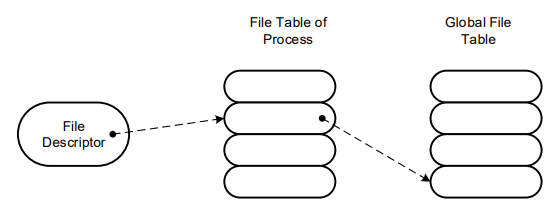
\includegraphics[scale = 0.25]{grafiken/filedescriptor.PNG}
%\prgc{STDIN_FILENO = 0}: standard input, \prgc{STDOUT_FILENO = 1}: standard output, \prgc{STDERR_FILENO = 2}, standard error

\subsubsection{POSIX API}
alle Daten sind rohe Binärdaten (wie abgespeichert)
%//kopiert 32 ersten Bytes von Datei in andere
%#define N 32
%char buf[N];
%char spath[PATH_MAX];
%char dpath[PATH_MAX];
%/* get paths from somewhere */
%int src = open(spath, O_RDONLY);
%int dst = open(dpath, O_WRONLY | O_CREAT, S_IRWXU);
%ssize_t read_bytes = read(src, buf, N);//->Anz. Bytes
%Write(dst, buf, read_bytes);
%close(src);
%Close(dst);
\begin{minted}{C}
lseek (fd, offset, origin) //return status
//Offset des FDs auf offset setzen
pread(..)/pwrite(..)
//mit Offset-Angabe, verändern FD nicht
\end{minted}

\subsubsection{C API}
formatierte Ein- und Ausgabe (via Streams(= \prgc{FILE})),
\textbf{File-Position-Indicator:} gepuffert $\rightarrow$ bestimmt Position im Puffer, ungepuffert $\rightarrow$ Offset des File-Descriptors
%\begin{minted}{c}
% FILE * src = fopen("path", "r");//O_RDONLY
% FILE * dest = fopen("path", "w");
% //O_WRONLY, O_CREAT, O_TRUNC
% //ein Byte schreiben:
% int temp = fgetc(src);
% fputc(temp, dest);
% fclose(src);
% fclose(dest);

%FILE *stdin, *stdout, *stderr
%fdopen(fd, const char* mode);//->FILE*
%fileno(FILE* stream);//->File-Descrip.
%fflush(FILE* stream);//Buffer leeren
%feof(stream);//0 = Ende nicht erreicht
%ferror(stream);//0 = kein Fehler
%fgetc(stream);//nächstes Byte als int z.
%fgets(string, stream)
%//bis Zeilenumbruch oder n-1 Bytes gelesen
%fputc(int c, stream)
%fputs(String, stream)
%fungetc(c, stream) 
%//schiebt c zurück in Stream 
%ftell(stream)//Indicator zurück
%fseek(...) //analog lseek
%rewind(stream)//stream zurücksetzen
%\end{minted}













